\bghdr{images/fond-win}

%\begin{center}
%
\includegraphics{images/logo_Windows}
%\end{center}


\subsection{Configuration sous Microsoft Windows}


Cette section d\'ecrit comment configurer un ordinateur tournant sous Windows XP, Windows Vista, Windows 7 ou Windows 8. Si tu poss\`edes une autre version de Windows,
nous t'invitons \`a  regarder directement la section sur les licences MSDNAA en page \pageref{msdnaa}\dots ou alors \`a  te d\'ebrouiller ! ;-)

\subsubsection{Configuration IP}

\begin{itemize}

\item \textbf{Sous Windows XP :} va dans le \menu{Menu D\'emarrer}, \menu{Panneau de configuration} et double-clique sur \menu{Connexions r\'eseau} puis sur \menu{Connexion au r\'eseau local}. Clique enfin sur \menu{Propri\'et\'es}.

\item \textbf{Sous Windows Vista :} va dans le \menu{Menu D\'emarrer}, \menu{Panneau de configuration}, \menu{R\'eseau et Internet}, \menu{Centre r\'eseau et partage}. L\`a, dans le menu \`a  gauche, clique sur \menu{G\'erer les connexions r\'eseau}, puis clique droit sur \menu{Connexion au r\'eseau local} et enfin  \menu{Propri\'et\'es}~\footnote{\`A ce stade, ainsi qu'\`a  plusieurs autres \'etapes de ce tutoriel, Windows Vista doit normalement t'afficher un message te demandant de confirmer l'action que tu viens d'effectuer. Donc tu confirmes, et cela \`a  chaque fois !}.

\item \textbf{Sous Windows 7 et Windows 8 :} va dans le \menu{Menu D\'emarrer} (Windows 7) ou le \menu{Menu Param\`etres} (Windows 8), \menu{Panneau de configuration}, \menu{R\'eseau et Internet}, \menu{Centre r\'eseau et partage}, \menu{Modifier les param\`etres de la carte}. Puis clique droit sur \menu{Connexion au r\'eseau local} et enfin  \menu{Propri\'et\'es}.

\end{itemize}



%\flimage{images/win_connexion_icone}{0.15}{l} Va dans le \menu{Menu
%D\'emarrer}, \menu{Panneau de configuration} et double-clique sur
%\menu{Connexions r\'eseau} puis sur \menu{Connexion au r\'eseau local}.
%Clique enfin sur \menu{Propri\'et\'es}.\\

%Dans cette fen\^etre, coche les trois cases \menu{Client pour les
%r\'eseaux Microsoft}, \menu{Partage de fichiers} et \menu{Protocole
%Internet (TCP/IP)}:

\imagepos{images/win_config_connexion2}{0.5}{Configurer la connexion au r\'eseau local}{!h}



%\imageref{images/win_config_ip}{0.5}{Configuration IP --- Propri\'et\'es de protocole Internet (TCP/IP)}{!ht}{config:win:IP1}
%%%%\imageref{images/win_config_ip2}{0.71}{Configuration de la connexion
%au r\'eseau local et propri\'et\'es du TCP/IP}{!ht}{config:win:IP1}

S\'electionne ensuite la ligne \menu{Protocole Internet Version 4 (TCP/IPv4)}~\footnote{\menu{Protocole Internet (TCP/IP)} pour certaines versions de Windows XP.},
puis clique sur le bouton \menu{Propri\'et\'es} qui vient de se
d\'egriser. Tu tombes alors sur l'\'ecran de configuration de ta
connexion vers l'ext\'erieur.

\noindent
  \begin{figure*}[!h]
    \begin{center}  
      \subfloat[Configuration IP --- Propri\'et\'es de protocole Internet (TCP/IP)]{ 
      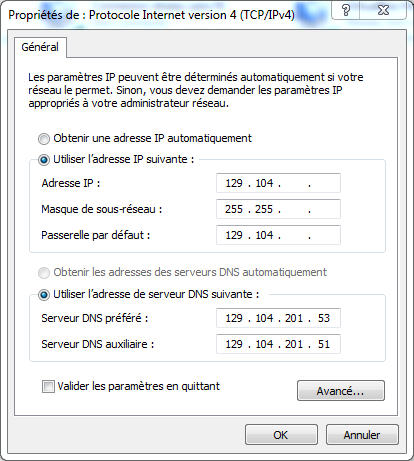
\includegraphics[width=0.48\textwidth]{images/win_config_ip} \label{config:win:IP1}}
      \hspace{\stretch{1}}
      \subfloat[Configuration DNS]{ 
         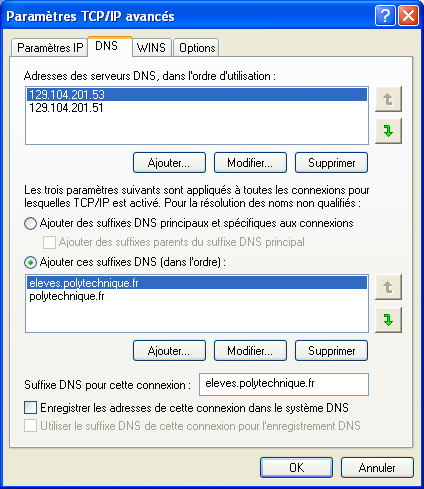
\includegraphics[width=0.48 \textwidth]{images/win_config_dns2} \label{config:win:IP2}}
             \caption{Configuration r\'eseau}
    \end{center}
  \end{figure*}



%% \newpage
Coche alors les cases \menu{Utiliser l'adresse IP suivante} et \menu{Utiliser l'adresse de serveur DNS suivante} et remplis les cinq champs d'adresse IP. Tu trouveras toutes les valeurs d'adresse IP n\'ecessaires pour la configuration en page~\pageref{tableau:mon_IP} ; aide-toi de la capture d'\'ecran~\ref{config:win:IP1} pour les placer. Si une partie d'adresse IP est blanche sur cette capture, c'est qu'elle t'est personnelle et que tu dois la calculer !
Clique ensuite sur le bouton \menu{Avanc\'e}, puis sur l'onglet
\menu{DNS} en haut.
Il n'y a plus qu'\`a  remplir les diff\'erents champs comme sur la
capture d'\'ecran suivante, avec le bouton \menu{Ajouter} et les
fl\`eches pour r\'eordonner les \'el\'ements.


%\subsubsection{Le domaine Windows}

%\paragraph{Qu'est ce que c'est ?}
%Le domaine Windows est un syst\`eme d'automatisation de la
%configuration de plusieurs ordinateurs sous Windows situ\'es sur le
%m\^eme r\'eseau. En fait, c'est un outil d'administration, con\c{c}u par
%exemple pour des entreprises o\`u un service informatique doit g\'erer
%de nombreuses machines; il permet d'appliquer des modifications de
%configuration \`a  toutes les machines du domaine directement depuis un
%serveur. Le BR poss\`ede un serveur d\'edi\'e au domaine Windows,
%\server{enez}.

%Le domaine met \`a  jour automatiquement Windows et l'antivirus \`a  partir d'\server{enez} (tr\`es rapide car tu n'as pas besoin de r\'ecup\'erer des fichiers
%en dehors de l'\'ecole!). Il configure le \emph{firewall} (pare-feu: syst\`eme de protection contre les \'eventuelles attaques par le r\'eseau) Windows, mais
%il est toujours possible de le d\'esactiver si tu pr\'ef\`eres un autre \emph{firewall}. En bref, il permet de simplifier \`a  l'extr\^eme %la mise \`a  jour
%continuelle de l'ordinateur.%


%\paragraph{Alors, domaine ou pas domaine ?} Soit tu choisis de te
%mettre sur le domaine Windows, et tu vas alors au paragraphe
%\guillemotleft~Inscription sur le domaine Windows~\guillemotright.%

%% \newpage
%\textbf{Avantages :}
%\begin{itemize}
%\item Windows est mis \`a  jour automatiquement ; tu as toujours les
%derni\`eres corrections de s\'ecurit\'e et un pare-feu correctement
%configur\'e. Donc tu es mieux prot\'eg\'e contre les intrusions.
%\item Surtout, tu n'as plus \`a  t'en occuper, presque tout est automatique.
%\end{itemize}%

%\textbf{Inconv\'enients :}
%\begin{itemize}
%  \item Tu d\'el\`egues une partie des droits d'administration de ta machine au BR
%        (tout ce qui concerne la s\'ecurit\'e du r\'eseau en particulier).
%        Cependant, si tu ne sais pas le faire, c'est plut\^ot un avantage
%        de laisser le BR s'en occuper \`a  ta place.
%  \item Cela ne marche qu'avec Windows 2000, Windows XP Pro ou Windows Vista Business.
%        On te rappelle que tu peux facilement, gratuitement et l\'egalement passer \`a 
%        Windows XP Pro ou bien \`a  Windows Vista Business (section sur les licences
%        MSDNAA en page \pageref{msdnaa}).
%\end{itemize}

%Bien s\^{u}r, tu peux sortir du domaine \`a  tout instant, et effectuer manuellement les r\'eglages n\'ecessaires \`a  la s\'ecurit\'e de ton ordinateur.

%Soit tu choisis de configurer toi-m\^eme ton ordinateur, et tu peux passer
%directement \`a  la section \guillemotleft Installation de l'antivirus
%\guillemotright. Tu trouveras les informations n\'ecessaires \`a  la configuration
%manuelle du pare-feu et du proxy pour \app{Windows Update} en annexe \`a  la
%fin de cette section, en page \pageref{horsdomaine}.

%\textbf{Avantage :} Tu es le seul \`a  t'occuper de la gestion de ton ordinateur.

%\textbf{Inconv\'enient :} Tu es le seul \`a  t'occuper de la gestion de ton ordinateur. ;-)
%S'il devient un foyer pour virus, sache que nous avons les moyens de l'isoler
%pour \'eviter toute propagation.

%\begin{center}
%  \fbox{
%    \begin{minipage}{.7\textwidth}
%      \begin{center}
%Le BR te conseille \emph{tr\`es fortement} de te mettre sur le domaine
%et de choisir l'installation simplifi\'ee !
%      \end{center}
%    \end{minipage}
%  }
%\end{center}


%\paragraph{Inscription sur le domaine Windows}

%On te rappelle que tu ne peux t'inscrire sur le domaine que si tu utilise
%Windows 2000, Windows XP Pro ou Windows Vista. Si tu poss\`ede Windows XP
%Familial, Windows Vista Home ou encore une version ant\'erieure de Windows,
%tu dois effectuer toi-m\^eme tes r\'eglages de pare-feu et de proxy
%\app{Windows Update}. R\'ef\`ere-toi pour cela \`a  l'annexe ad hoc \`a  la fin de
%cette section, en page \pageref{horsdomaine}.

%La proc\'edure d'inscription est la suivante :
%\begin{itemize}

%\item \textbf{Sous Windows XP :} Clique sur le \menu{Menu D\'emarrer} puis fais un clic-droit sur
%\menu{Poste de travail} et choisis \menu{Propri\'et\'es}. Ensuite, s\'electionne l'onglet \menu{Nom de l'ordinateur} et clique le bouton \menu{Modifier}.

%\item \textbf{Sous Windows Vista :} Clique sur \menu{Menu D\'emarrer}, puis fais un clic-droit sur \menu{Ordinateur}, \menu{Propri\'et\'es}. L\`a  s\'electionne \menu{Param\`etres syst\`eme avanc\'es}, onglet \menu{Nom de l'ordinateur}, puis clique sur le bouton \menu{Modifier}.

%\end{itemize}

%Dans la case \menu{Nom de l'ordinateur}, rentre ton pseudo, puis coche la case \menu{domaine} et
%rentre \urllink{windows.eleves.polytechnique.fr}. Note bien que l'inscription au domaine te sera
%refus\'ee par le serveur si quelqu'un d'autre utilise d\'ej\`a  le m\^eme nom d'ordinateur que toi. Par
%cons\'equent, essaie d'opter pour un pseudo qui t'identifie de fa\c{c}on claire et unique, par exemple
%\cmd{NOM\_PRENOM} \footnote{Les Jean Dupont et les Julien Thomas sont pri\'es de trouver autre chose
%;-)}.

%\imagepos{images/win_config_domaine}{0.5}{S'inscrire sur le domaine windows}{!ht}

%\begin{center}
%\begin{tabular}{ll}
% \parbox{.45\textwidth}{
%  et si tu es rouje 2006 :
%  \begin{description}
%    \item[Nom] rouje06
%    \item[Mot de passe] rouje.2006
%  \end{description}
 % }
% & \parbox{.45\textwidth}{
%  Si tu es j\^one 2007, tu rentres :
%  \begin{description}
%    \item[Nom] jone07
%    \item[Mot de passe] jone.2007
%  \end{description}
%  }
%\\
%\end{tabular}
%\end{center}

%\emph{Attention, ces identifiants servent juste \`a  t'inscrire sur le
%domaine. Pour utiliser ton ordinateur, tu devras rentrer au
%d\'emarrage les m\^emes nom d'utilisateur et mot de passe que tu avais
%avant d'\^etre sur le domaine !}
%
%
%
%%\paragraph{Installation personnalis\'ee} --- configuration manuelle

%\subparagraph{Configuration antivirus} Le BR, concern\'e par la
%s\'ecurit\'e du r\'eseau, te propose un antivirus pour lequel tu n'auras
%pas \`a  payer la license pour obtenir les mises \`a  jour. Bien s\`a�¿½r,
%libre \`a  toi d'utiliser ton anti-virus personnel ; cependant il sera
%\`a  ta charge de le mettre \`a  jour tr\`es r\'eguli\'erement. Pour cela
%utilise comme proxy : \urllink{http://kuzh} sur le port 8080.

%\emph{Installation de l'anti-virus du BR}\ : Commence par
%d\'esinstaller tous les antivirus ou firewalls que tu pourrais avoir
%comme expliqu\'e dans le paragraphe \guillemotleft~Installation simplifi\'ee
%--- configuration automatique~\guillemotright .

%Puis ouvre ton explorateur Windows et tape :
%\urllink{$\backslash\backslash$enez$\backslash$antivirus}
%et double-clique sur le fichier \file{Symantec.exe}.

%Ce package contient le param\'etrage de la mise \`a  jour automatique de
%Windows sur le serveur de l'\'ecole. Attends la fin de l'installation
%et c'est fini ! Maintenant, tu n'as plus \`a  toucher \`a  l'antivirus,
%normalement il sera mis \`a  jour automatiquement.

%\subparagraph{Configuration firewall}

%Si tu as Windows XP avec le SP2 install\'e, tu as un firewall
%automatiquement activ\'e et facile d'utilisation. En effet, \`a  chaque
%fois qu'un programme tentera d'aller pour la premi\`ere fois sur
%Internet, il te demandera si tu veux le laisser faire ou non, comme
%dans la capture~\ref{config:win:firewall}.

%\imageref{images/win_firewall}{0.8}{Un programmme --- ici GuildFTP
%--- demande \`a  acc\'eder au r\'eseau}{!ht}{config:win:firewall}

%Le firewall commercial \app{ZoneAlarm}, ind\'ependant de Windows,
%fonctionne sur le m\^eme principe. Tu peux le trouver sur \xshare.

%Si tu pr\'ef\`eres utiliser le firewall int\'egr\'e \`a  Windows XP (sans le
%SP2) ou \`a  Windows Server 2003, il te faudra le configurer en d\'etail.
%Va dans le \menu{Menu D\'emarrer}, \menu{Param\`etres} et clique sur
%\menu{Connexions R\'eseau}. Choisis la connexion qui est utilis\'ee par
%ton ordinateur (souvent il n'y en a qu'une, ou alors une seule est
%activ\'ee) et double-clique dessus. Clique sur \menu{Propri\'et\'es} en
%bas \`a  gauche, puis sur l'onglet \menu{Avanc\'e} et rentre dans le menu
%de \menu{Param\`etres} du \menu{Pare-feu Windows}. Il te faudra alors
%ajouter manuellement tous les ports que tu veux ouvrir sur
%l'ext\'erieur. Pour cela, clique sur \menu{Ajouter}, et remplis la
%bo\`a�¿½te de dialogue en t'aidant de la capture
%d'\'ecran~\ref{config:win:ouvrir_port}; mets le num\'ero du port que tu
%veux ouvrir, par exemple 5050, 5053 et 5055 en TCP pour \app{qRezix}
%et 21 en TCP pour ton FTP.

%\imageref{images/win_config_firewall}{0.7}{Ouvrir un port dans le firewall %Windows}{!ht}{config:win:ouvrir_port}

%Comme tu peux le constater, il est beaucoup plus pratique d'aller
%sur le domaine et de laisser le SP2 faire le gros du boulot \`a  ta
%place :-).



\subsubsection{Configuration \emph{web} (serveur mandataire)}

\imageref{images/win_config_proxy}{0.5}{Configuration du serveur mandataire (\emph{proxy})}{!ht}{config:win:proxy}

M\^eme si tu n'utilises pas \app{Internet Explorer} comme client \emph{web}, Windows et d'autres programmes
utilisent ses param\`etres, notamment \app{Windows Update}. Par conséquent lance \app{Internet Explorer} et va
dans le menu \menu{Outils}, \menu{Options Internet}, puis sur l'onglet \menu{Connexions} de la
nouvelle fen\^etre et enfin sur \menu{Param\`etres r\'eseau} dans le bas de la fen\^etre. Tu dois \^etre arriv\'e sur une fen\^etre semblable \`a celle de la capture d'\'ecran~\ref{config:win:proxy}. L\`a, coche
uniquement la case \menu{Utiliser un script de configuration automatique}, puis remplis le champ
\menu{Adresse} avec \urllink{http://config/proxy.pac}.

Une fois que tu as fait \c{c}a, tu n'as plus forc\'ement besoin d'\app{Internet Explorer}, tu peux donc utiliser un autre navigateur, comme \app{Mozilla
Firefox}, disponible sur \urllink{http://www.mozilla-europe.org/fr/products/}.

Même si tu ne configures pas Windows Update avec le paragraphe ci-dessous, n'oublie pas de régler ton navigateur \emph{web} et ton client \emph{mail} si tu en as un : reporte-toi page \pageref{browser}.

\subsubsection{Windows Update}

\label{horsdomaine} %\emph{Cette sous-section ne concerne pas les gens qui ont choisi de s'inscrire sur le domaine.}

%\paragraph{Pare-feu} Si tu as Windows XP avec le SP2 install\'e, ou \emph{a fortiori}
%Windows Vista, tu as un \emph{firewall} automatiquement activ\'e et facile d'utilisation. En effet, \`a  chaque fois qu'un programme tentera d'aller pour
%la premi\`ere fois sur Internet, il te demandera si tu veux le laisser faire ou non. Si tu pr\'ef\`eres une protection ind\'ependante de Windows, le
%\emph{firewall} commercial \app{Zone\-Alarm} fonctionne sur le m\^eme principe. Tu peux le trouver sur \xshare.

%Si tu pr\'ef\`eres utiliser le \emph{firewall} int\'egr\'e \`a  Windows XP (sans le SP2), il te faudra le configurer en d\'etail. Va dans le \menu{Menu D\'emarrer},
%\menu{Param\`etres} et clique sur \menu{Connexions R\'eseau}. Choisis la connexion qui est utilis\'ee par ton ordinateur (souvent il n'y en a qu'une, ou
%alors une seule est activ\'ee) et double-clique dessus. Clique sur \menu{Propri\'et\'es} en bas \`a  gauche, puis sur l'onglet \menu{Avanc\'e} et rentre dans le
%menu de \menu{Param\`etres} du \menu{Pare-feu Windows}. Il te faudra alors ajouter manuellement tous les ports que tu veux ouvrir sur l'ext\'erieur. Pour
%cela, clique sur \menu{Ajouter}, et remplis la bo\^ite de dialogue% en t'aidant de la capture d'\'ecran~\ref{config:win:ouvrir_port} ci apr\`es
%; mets le num\'ero du port que tu veux ouvrir, par exemple 5050, 5053 et 5055 en TCP pour \app{qRezix} et 21 en TCP pour ton FTP.

Il reste une derni\`ere configuration de
serveur mandatataire indispensable pour que puissent se faire les mises \`a  jour automatiques
de Windows. Il t'est fortement recommand\'e de le faire.

\begin{description}

\item[Sous Windows 7 \& Windows 8] Si tu as correctement configuré ton serveur \emph{web} mandataire, les mises à jours se font automatiquement.

\item[Sous Windows XP] Fais \menu{D\'emarrer}, \menu{Ex\'ecuter}, puis
tape \cmd{cmd} dans la fen\^etre qui s'affiche. Une ligne de commande apparaît,
il te suffit alors de taper : \cmd{proxycfg -p http://kuzh:8080} pour r\'egler
le serveur mandataire. Pour revenir \`a  un acc\`es direct il faut taper \cmd{proxycfg -d}.

\item[Sous Windows Vista]
Dans le menu \menu{D\'emarrer}, tape \guillemotleft~Invite de commandes~\guillemotright{} dans le champ \menu{Rechercher}, puis clique droit sur le lien
et choisis \menu{Ex\'ecuter en tant qu'administrateur}. Tape ensuite les commandes suivantes :
\cmdline{
C:\textbackslash{}Windows\textbackslash{}system32$>$netsh\\
netsh>winhttp\\
netsh winhttp>set proxy proxy-server="http://kuzh:8080"\\
netsh winhttp>exit\\
C:\textbackslash{}Windows\textbackslash{}system32>exit }

Pour revenir à l'accès direct, il suffit de taper :
\cmdline{
  netsh winhttp reset proxy
}

Pour la suite de ta configuration, rendez-vous page \pageref{browser} pour faire marcher ton navigateur web préféré !

\end{description}

\clearpage
